\begin{figure*}
\vspace{-1.5em}

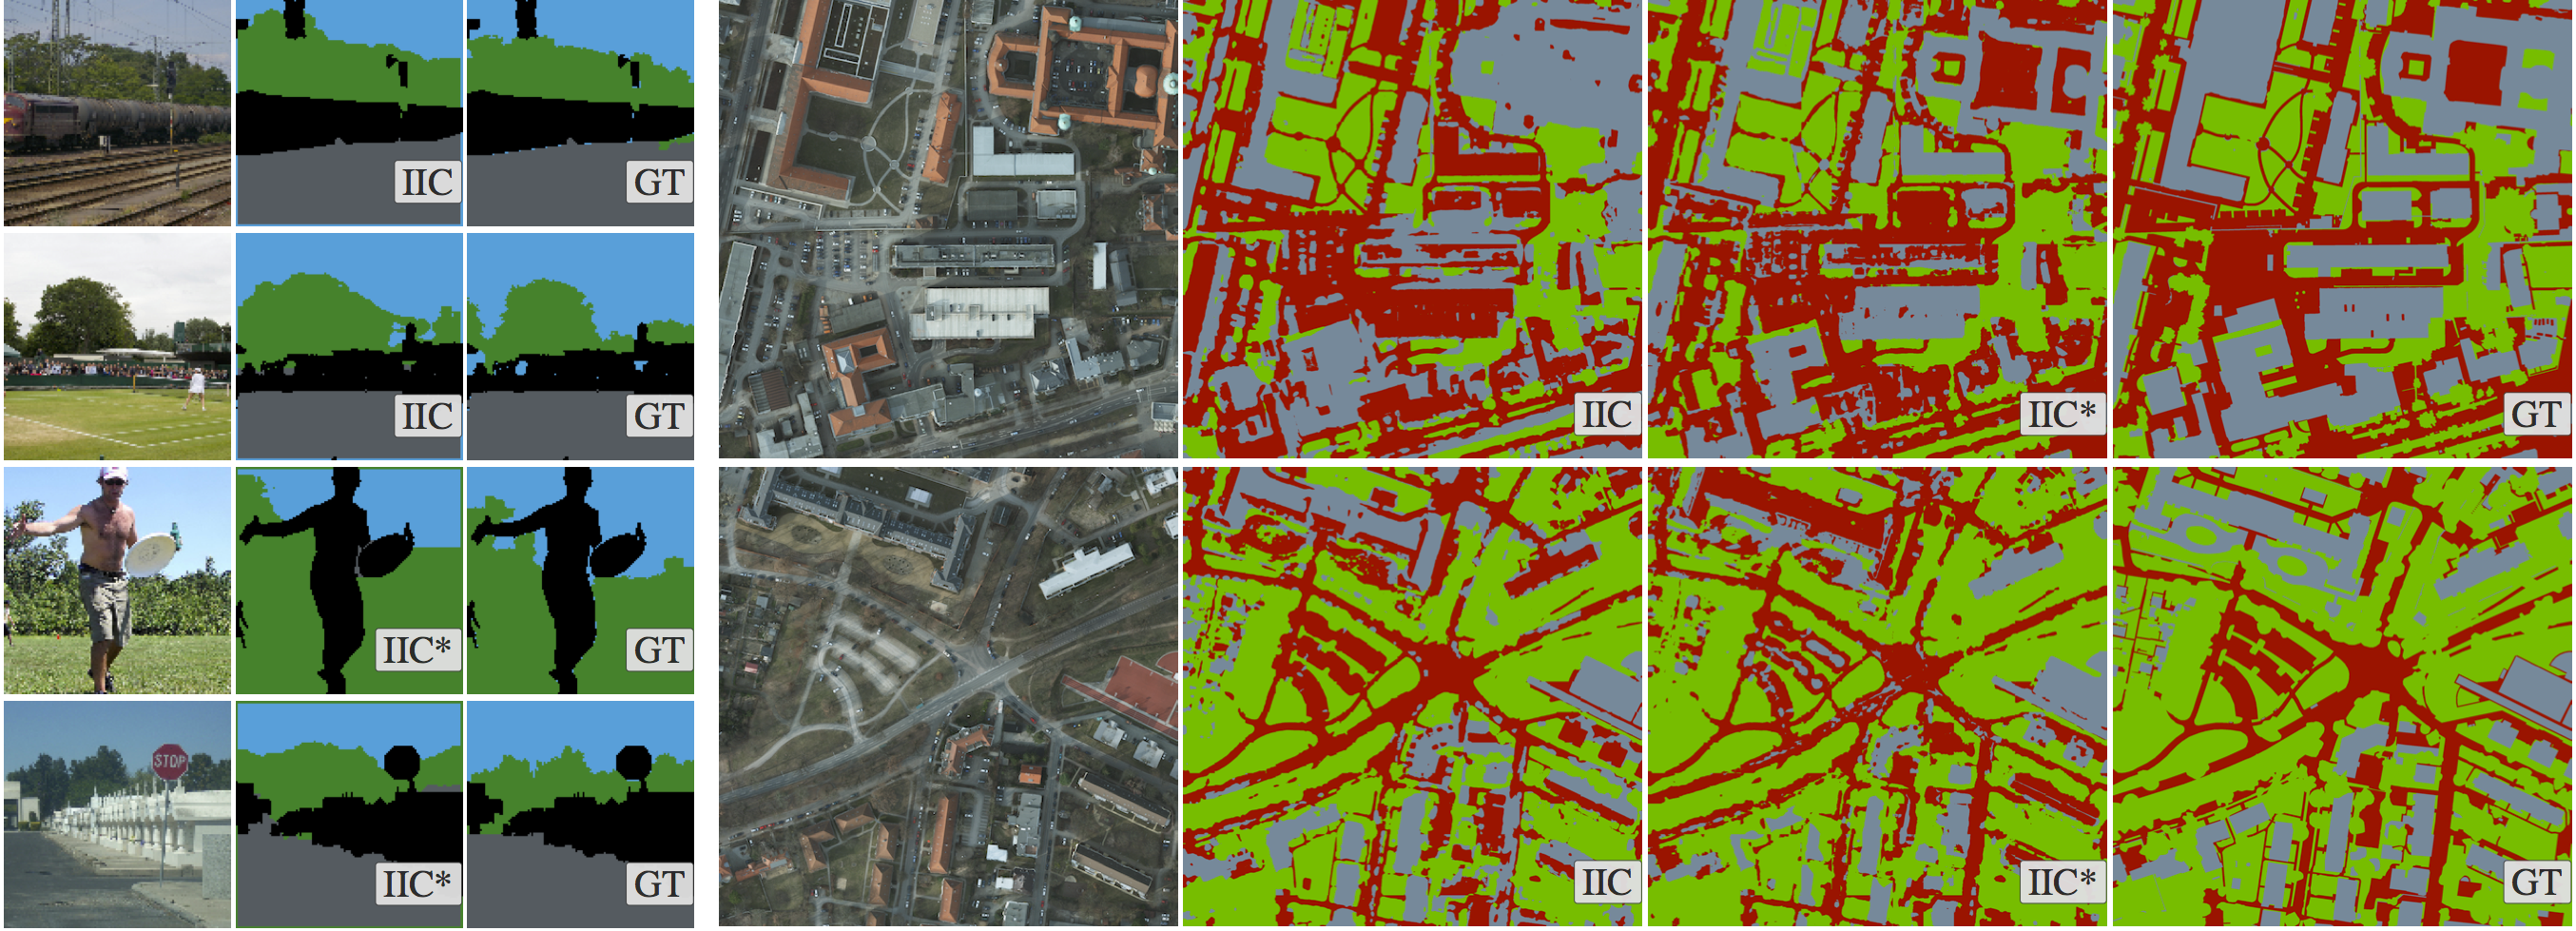
\includegraphics[width=\textwidth]{experiments2_files/fig-7-orig.png}

\caption{\textbf{Example segmentation results (un- and semi-supervised).} Left: COCO-Stuff-3 (non-stuff pixels in black), right: Potsdam-3. Input images, IIC (fully unsupervised segmentation) and IIC* (semi-supervised overclustering) results are shown, together with the ground truth segmentation (GT).}
%Left: COCO-Stuff-3, top two rows IIC, bottom two rows IIC+. Left to right: input, prediction, ground truth. Right: Potsdam-3. Left to right: input, IIC prediction, IIC+ prediction, ground truth.}
\label{f:images_img_seg}
\end{figure*}


\begin{comment}
\vspace{-2em}
\contourlength{1pt} %how thick each copy is
\contournumber{40}  %number of copies
\newcommand{\xput}[3]{%
% \begin{overpic}[#1]{#2}%
% \put (80,5) {\transparent{0.8}{\scriptsize{\colorbox{white}{#3}}}}%
% %\put (5,5) {\scriptsize\makebox(0,0){\contour{white}{#3}}}%
% %\put (5,5) {\scriptsize{\contour{white}{#3}}}%
% \end{overpic}
\includegraphics[#1]{#2}%
\raisebox{5pt}{\makebox[0pt][r]{%
%\transparent{0.8}{\contour{white}{\scriptsize #3\ }}}}}
%\transparent{0.8}{\colorbox{white}{\scriptsize #3}}}}}
\transparent{0.8}{\scriptsize\tcbox[colback=white,size=fbox,on line]{#3}}}}}
\begin{minipage}{0.27\textwidth}
\raggedright
\setlength\tabcolsep{1pt}
\renewcommand{\arraystretch}{0.8}
\begin{tabular}{ccc}
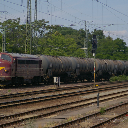
\includegraphics[height=0.32\textwidth]{experiments2_files/509_img_77.png} &
\xput{height=0.32\textwidth}{experiments2_files/509_reordered_preds_77.png}{IIC} &
\xput{height=0.32\textwidth}{experiments2_files/509_targets_77.png}{GT} \\
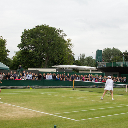
\includegraphics[height=0.32\textwidth]{experiments2_files/509_img_441.png}&
\xput{height=0.32\textwidth}{experiments2_files/509_reordered_preds_441.png}{IIC} &
\xput{height=0.32\textwidth}{experiments2_files/509_targets_441.png}{GT} \\
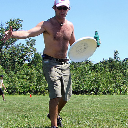
\includegraphics[height=0.32\textwidth]{experiments2_files/496_img_64.png} &
\xput{height=0.32\textwidth}{experiments2_files/496_reordered_preds_64.png}{IIC*} &
\xput{height=0.32\textwidth}{experiments2_files/496_targets_64.png}{GT}  \\
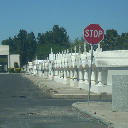
\includegraphics[height=0.32\textwidth]{experiments2_files/496_img_489.png} &
\xput{height=0.32\textwidth}{experiments2_files/496_reordered_preds_489.png}{IIC*} &
\xput{height=0.32\textwidth}{experiments2_files/496_targets_489.png}{GT} \\
\end{tabular}
\end{minipage}~%
\begin{minipage}{0.72\textwidth}
\raggedright
\setlength\tabcolsep{1.2pt}
\begin{tabular}{cccc}
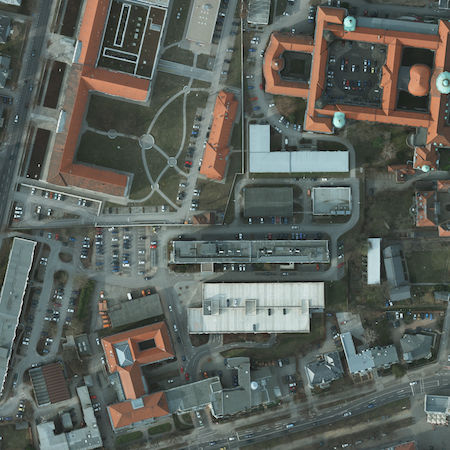
\includegraphics[height=0.243\textwidth]{experiments2_files/545_12_img.png} &
\xput{height=0.243\textwidth}{experiments2_files/545_12_preds.png}{IIC} &
\xput{height=0.243\textwidth}{experiments2_files/482_12_preds.png}{IIC*} &
\xput{height=0.243\textwidth}{experiments2_files/545_12_gt.png}{GT} \\
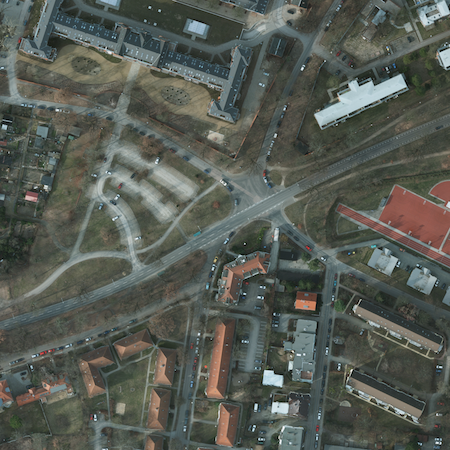
\includegraphics[height=0.243\textwidth]{experiments2_files/545_5_img.png} &
\xput{height=0.243\textwidth}{experiments2_files/545_5_preds.png}{IIC} &
\xput{height=0.243\textwidth}{experiments2_files/482_5_preds.png}{IIC*} &
\xput{height=0.243\textwidth}{experiments2_files/545_5_gt.png}{GT} \\
\end{tabular}
\end{minipage}
\end{comment}
